\begin{frame}{Model pekárny}
    \begin{block}{Vstupní tok}
    Do pekárny přicházejí zákazníci (\(\lambda =\)zákazníci za hodinu)
    \end{block}
    \begin{block}{Výstupní tok}
    \begin{itemize}
    \item počet pokladen
    \item střední doba obsluhy (\(\frac{\Delta t}{\mu}\))
    \end{itemize}
    \end{block}
    \begin{block}{Fronta}
    \begin{itemize}
    \item nekonečná
    \item FIFO
    \item střední doba trpělivosti (\(\tau\))
    \end{itemize}
    \end{block}
\end{frame}
\begin{frame}{Jedna realizace}
    \begin{figure}
\centering
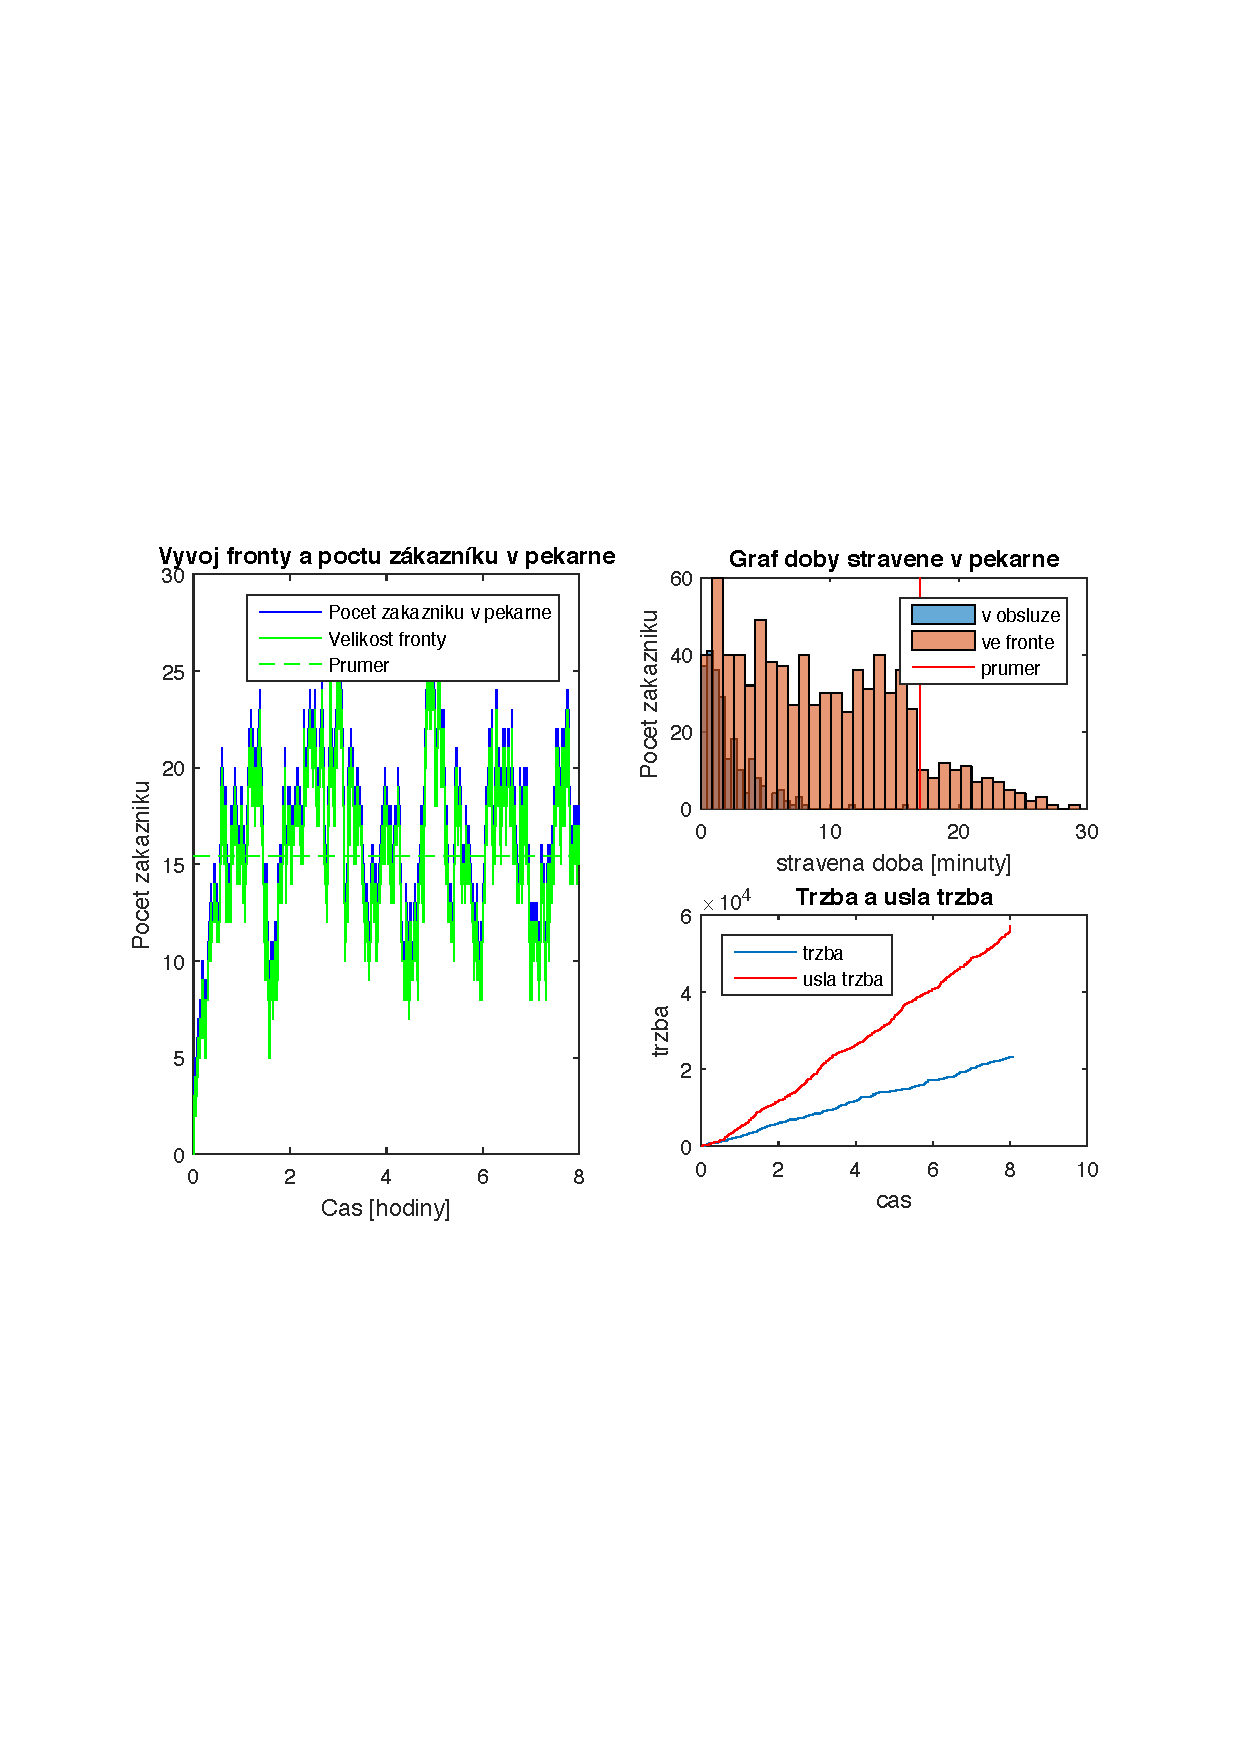
\includegraphics[width=0.8\columnwidth]{imgs/jedenPrubeh.pdf}
\label{fig:jedenPrubeh}
\caption{Simulace jedné osmihodinové směny v pekárně s jednou pokladnou.}
\end{figure}
\end{frame}
\begin{frame}{Jedna realizace}
    \begin{figure}
\centering
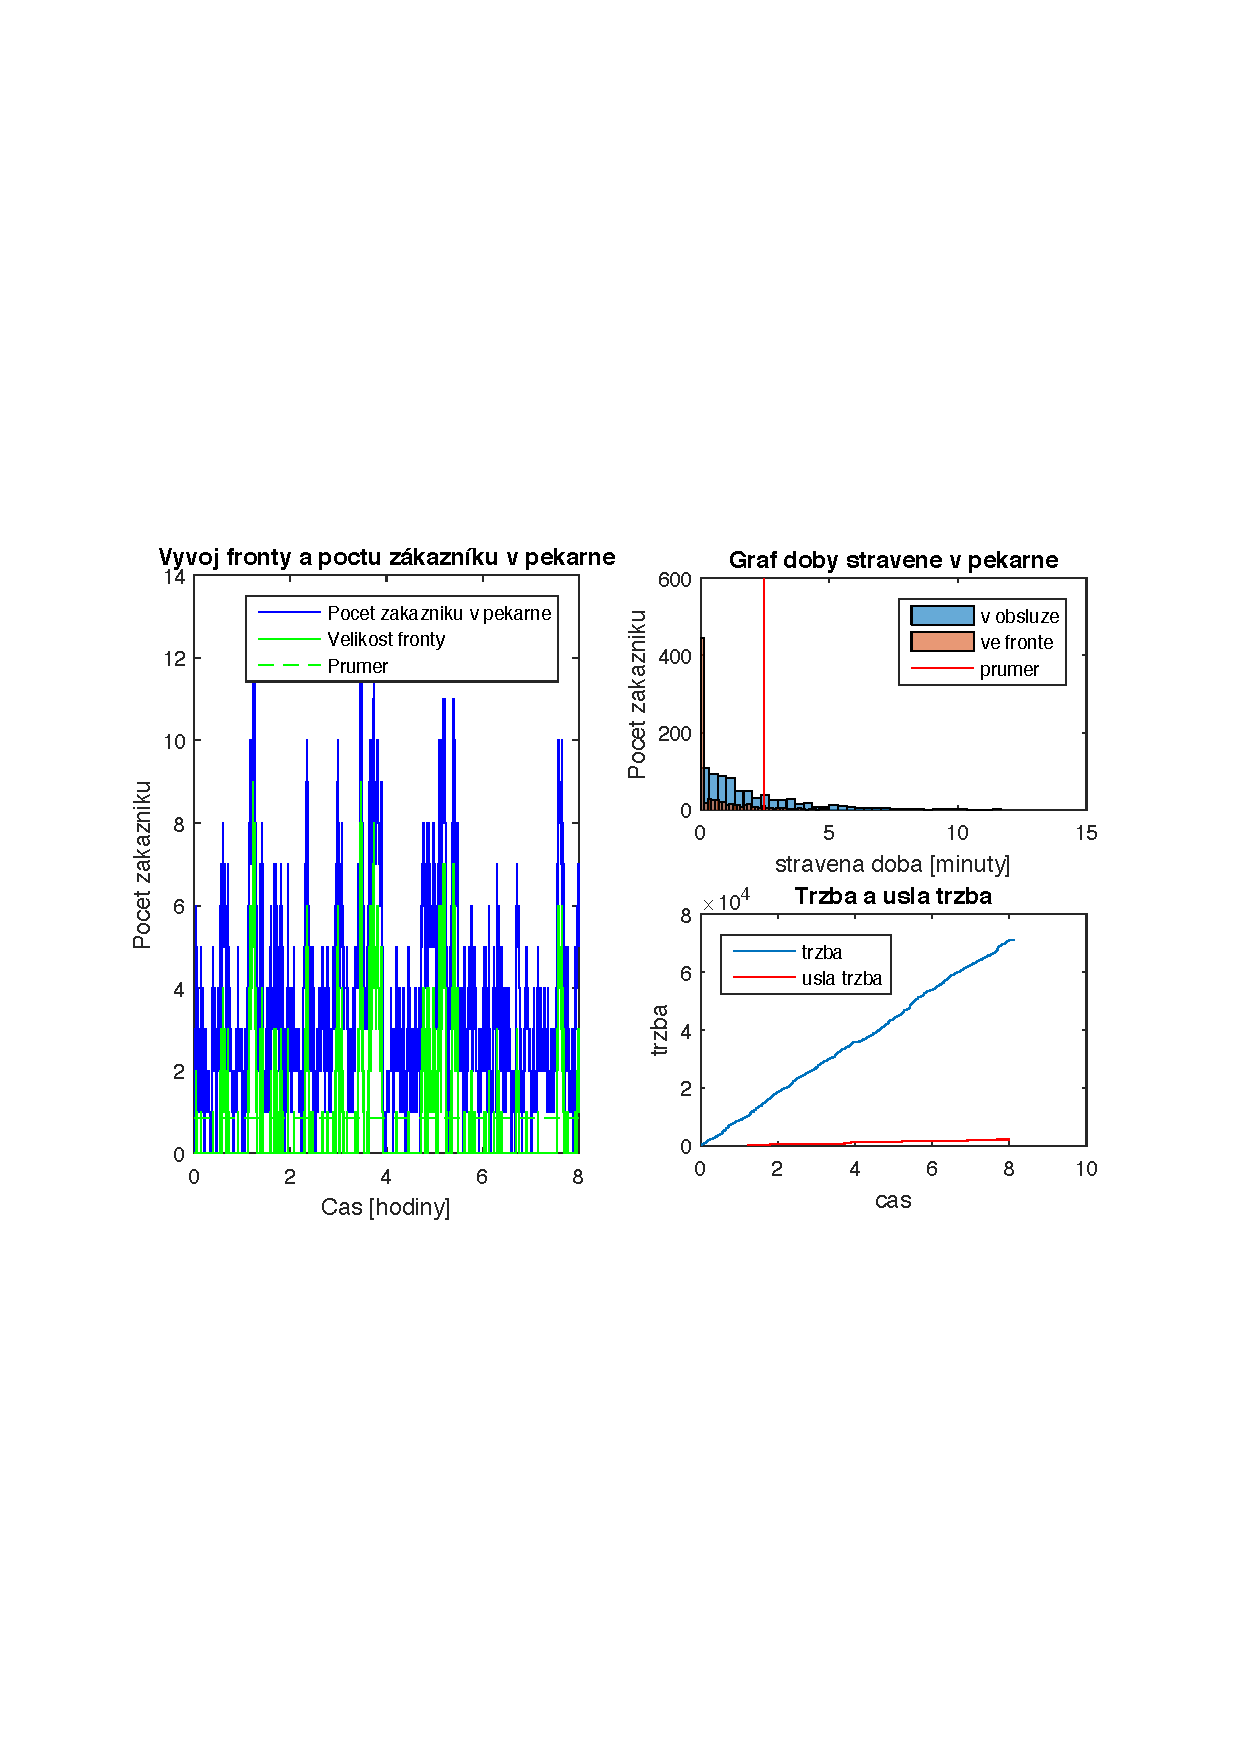
\includegraphics[width=0.8\columnwidth]{imgs/jedenPrubeh4.pdf}
\label{fig:jedenPrubeh4}
\caption{Simulace jedné osmihodinové směny v pekárně se 4 pokladnami.}
\end{figure}
\end{frame}
